\documentclass[10pt]{beamer}

\usepackage{color}
\usepackage{tikz}
\usepackage{mathtools}
\usepackage{array}
\usepackage{amsmath, amssymb, bbm}
\usepackage{verbatim}
\usepackage{relsize}
\usepackage{multirow}
\usepackage{rotating}
\usepackage{ragged2e}
\usetheme{Warsaw}
\usepackage{dsfont}
%\usecolortheme{lily}

\definecolor{obs}{RGB}{53,106,160}
\definecolor{post}{RGB}{0,110,46}
\definecolor{class}{RGB}{160,110,46}
\definecolor{idea}{RGB}{162,162,162}

\definecolor{gg1}{RGB}{248,118,109}
\definecolor{gg2}{RGB}{183,159,0}
\definecolor{gg3}{RGB}{0,186,56}
\definecolor{gg4}{RGB}{0,191,196}
\definecolor{gg5}{RGB}{97,156,255}
\definecolor{gg6}{RGB}{245,100,227}

\newcommand{\obs}[1]{{\color{obs}#1}}
\newcommand{\post}[1]{{\color{post}#1}}
\newcommand{\class}[1]{{\color{class}#1}}
\newcommand{\idea}[1]{{\uncover<2>{\color{idea}#1}}}
\newcommand{\tidea}[2]{{\uncover<#1>{\color{idea}#2}}}
\newcommand{\red}[1]{{\color{red}#1}}
\newcommand{\blue}[1]{{\color{blue}#1}}

\newcommand{\gga}[1]{{\color{gg1}#1}}
\newcommand{\ggb}[1]{{\color{gg2}#1}}
\newcommand{\ggc}[1]{{\color{gg3}#1}}
\newcommand{\ggd}[1]{{\color{gg4}#1}}
\newcommand{\gge}[1]{{\color{gg5}#1}}
\newcommand{\ggf}[1]{{\color{gg6}#1}}

\title{Merging classes}
\author{Marc Comas Cuf\'{\i}}
\date{}

\begin{document}


\begin{frame}
\titlepage
\end{frame}

%%% Introduction
\section{Mixture models}
\frame{\sectionpage}

\begin{frame}

\frametitle{Mixture models}
\begin{itemize}
\item A mixture model is a probability distribution with density function, $f$, defined as a linear combination of density functions, $f_1, \dots f_k$, coming from other probability distributions.
\[
f(x, \blue{\pi_1}, \dots, \blue{\pi_k}, \blue{\theta_1}, \dots, \blue{\theta_k}) = \blue{\pi_1} f_1(x, \blue{\theta_1}) + \dots + \blue{\pi_k} f_k(x, \blue{\theta_k})
\]
\item Given a  sample $X$, parameters $\blue{\pi_1}, \dots, \blue{\pi_k}, \blue{\theta_1}, \dots, \blue{\theta_k}$ can be estimated using the $EM$ algorithm.
\item $EM$-algorithm needs the number of components is fixed.
\end{itemize}
\end{frame}

\begin{frame}[t]
\frametitle{Mixture models: Gaussian example}
\begin{block}{Example: fitting a gaussian mixture}
Given a sample $X$ and setting the number of components to $6$. $EM$-algorithm can find the Gaussian mixture which fits ``better'' (with maximum likelihood) to sample $X$.
\end{block}
\medskip
\begin{columns}
\column{0.35\textwidth}%
\only<1>{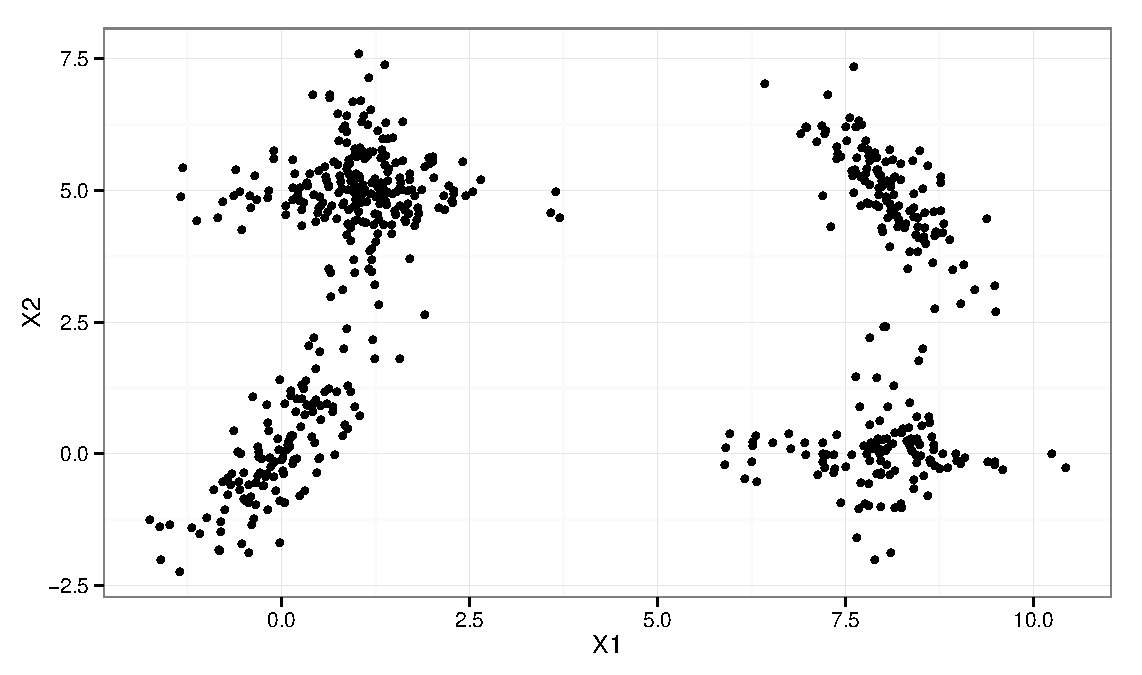
\includegraphics[width=\textwidth]{figures/baudry_ex4_1.pdf}}%
\only<2>{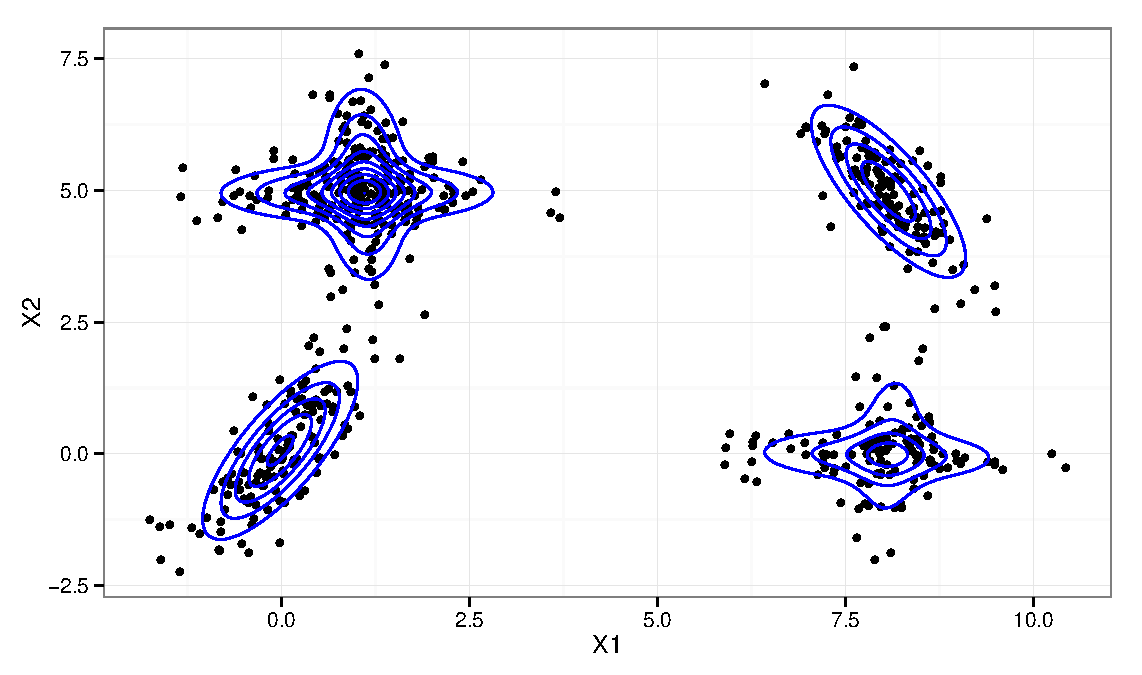
\includegraphics[width=\textwidth]{figures/baudry_ex4_1_contour6.pdf}}

\column{0.6\textwidth}
\uncover<2>{
{\tiny $\pi_1 = 0.12$, $\pi_2 = 0.20$, $\pi_3 = 0.19$, $\pi_4 =0.19$, $\pi_5 = 0.22$, $\pi_6 = 0.08$}

\noindent\rule{4cm}{0.4pt}

{\tiny $\mu_1 = (7.9, -0.02)$, $\mu_2 = (8.07, 4.98)$, $\mu_3 = (1.01, 4.96)$, $\mu_4 = (1.11, 5.12)$, $\mu_5 = (-0.02, 0.06)$, $\mu_6 = (8.10, 0.17)$}

\noindent\rule{4cm}{0.4pt}

{\tiny
$\Sigma_1 = \left(\begin{array}{cc}1.08 & -0.04\\ -0.04 & 0.10 \end{array}\right)$ 
$\Sigma_2 = \left(\begin{array}{cc}0.33 & -0.41\\ -0.41 & 0.85 \end{array}\right)$
$\Sigma_3 = \left(\begin{array}{cc}1.08 & 0.01\\ 0.01 & 0.10 \end{array}\right)$ 
$\Sigma_4 = \left(\begin{array}{cc}0.10 & -0.03\\ -0.03 & 1.08 \end{array}\right)$
$\Sigma_5 = \left(\begin{array}{cc}0.32 & 0.41\\ 0.41 & 0.86 \end{array}\right)$ 
$\Sigma_6 = \left(\begin{array}{cc}0.11 & 0.06\\  0.06 & 1.07 \end{array}\right)$
}
}
\end{columns}
\end{frame}


\begin{frame}
\frametitle{Mixture models: classifying observation}

\begin{itemize}
\item Adjusted density function:
\[
f(x) = \pi_1 \gga{f_1}(x) + \pi_2 \ggb{f_2}(x) + \pi_3 \ggc{f_3}(x) + \pi_4 \ggd{f_4}(x) + \pi_5 \gge{f_5}(x) + \pi_6 \ggf{f_6}(x)
\]
\item Any observation $x_i$ can be classified to component $j$ with maximimum
\begin{eqnarray*} \tau_{ij} &=& \frac{\pi_j f_j(x_i)}{f(x_i) } \end{eqnarray*}
\end{itemize}

\uncover<2->{%
\only<1-2>{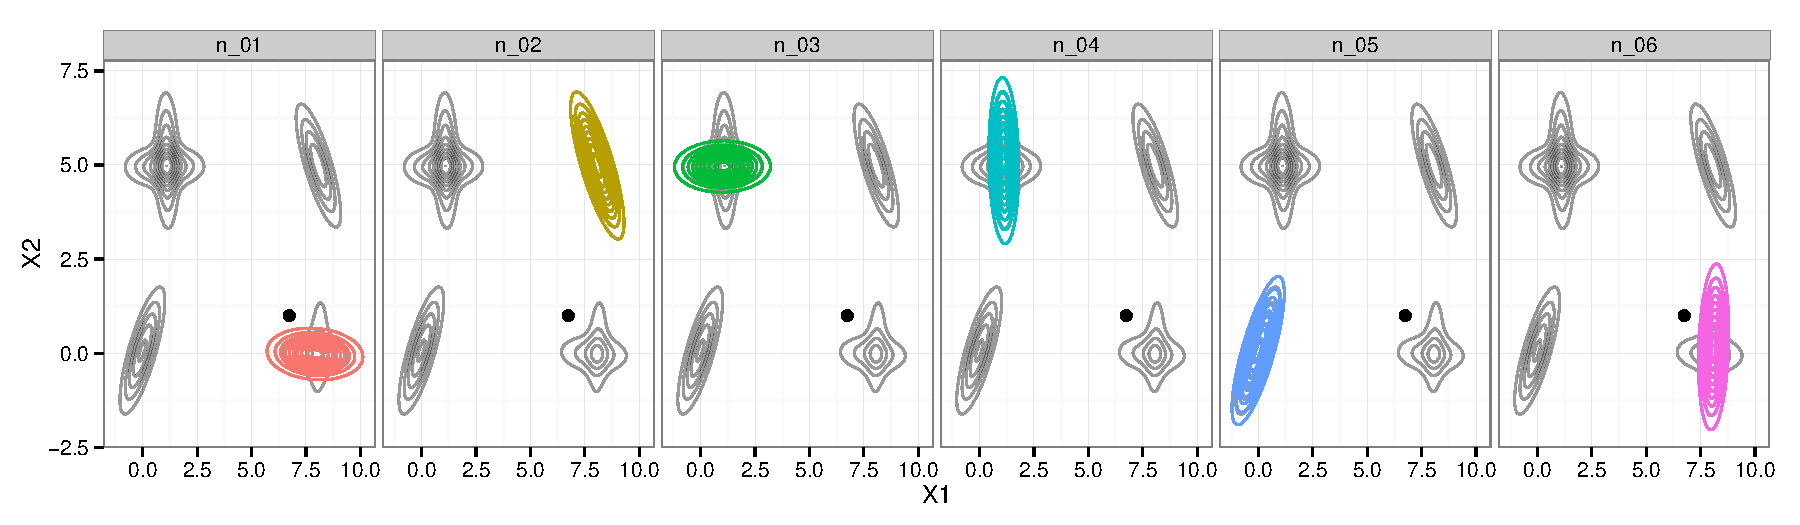
\includegraphics[width=\textwidth]{figures/baudry_ex4_1_all_distributions_one.pdf}}%
\only<3>{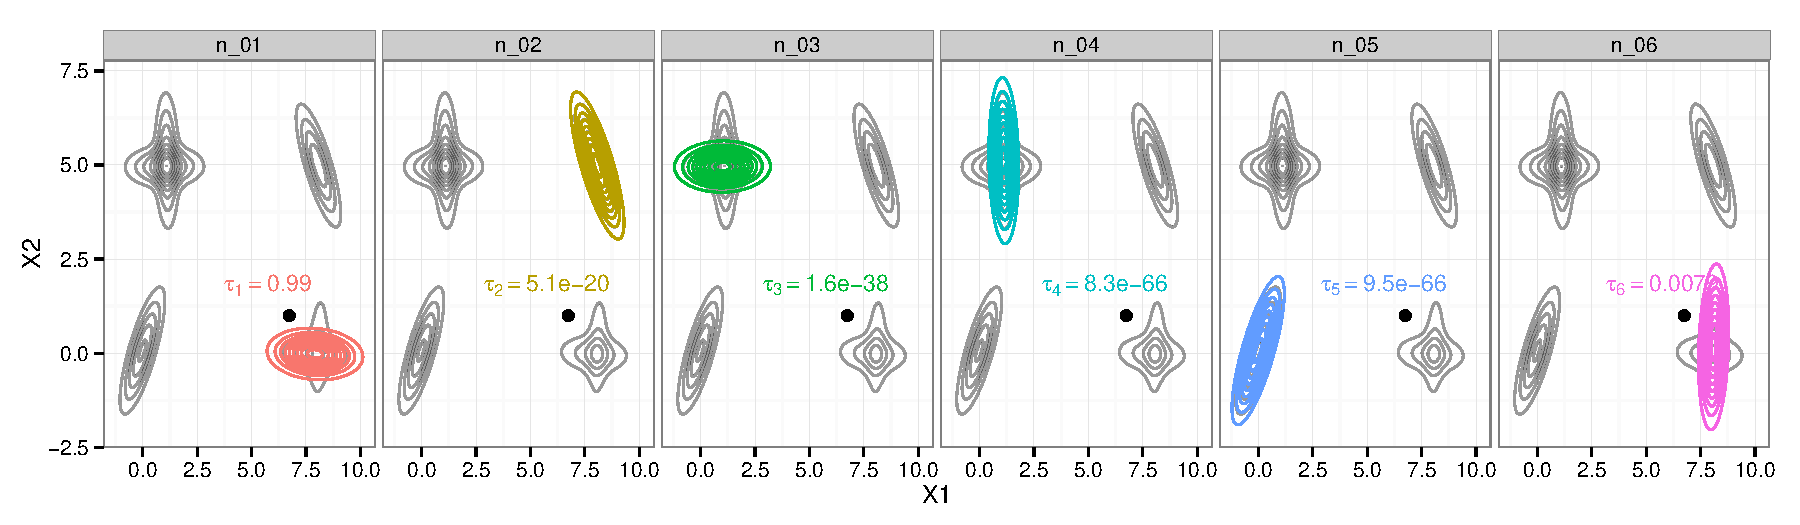
\includegraphics[width=\textwidth]{figures/baudry_ex4_1_all_distributions_one_tau.pdf}}}
\end{frame}

\begin{frame}
\frametitle{Mixture models: merging components}

\begin{columns}[T]
\column{0.4\textwidth}
\centering
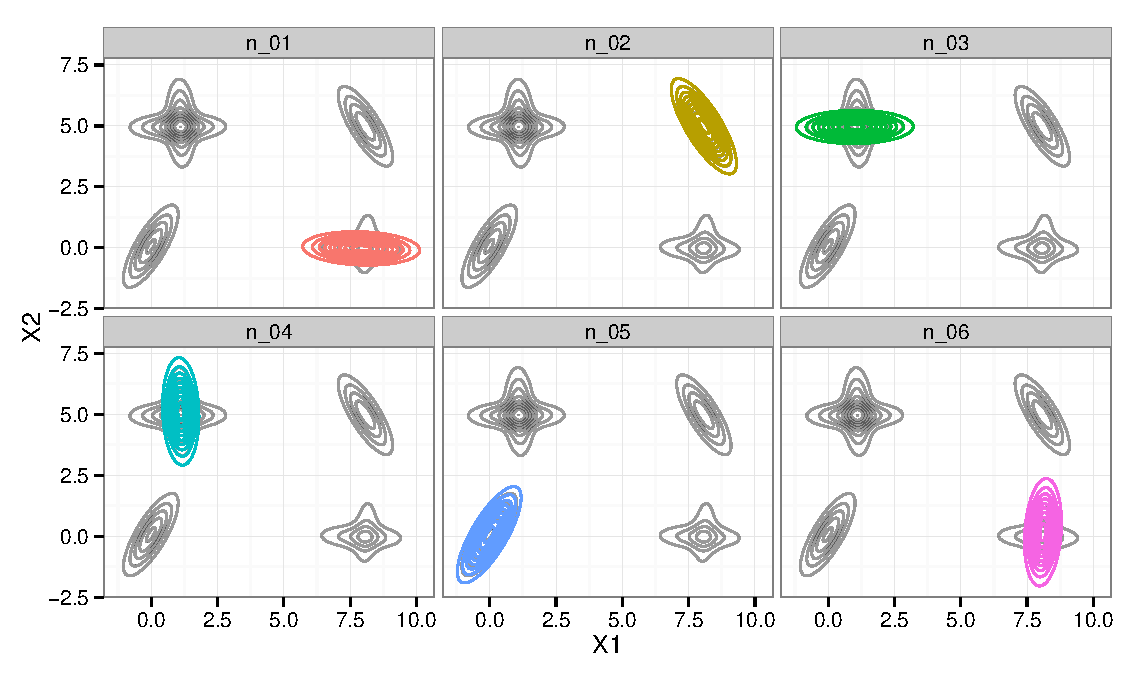
\includegraphics[width=0.9\textwidth]{figures/baudry_ex4_1_all_distributions.pdf}

\bigskip
\uncover<2->{%
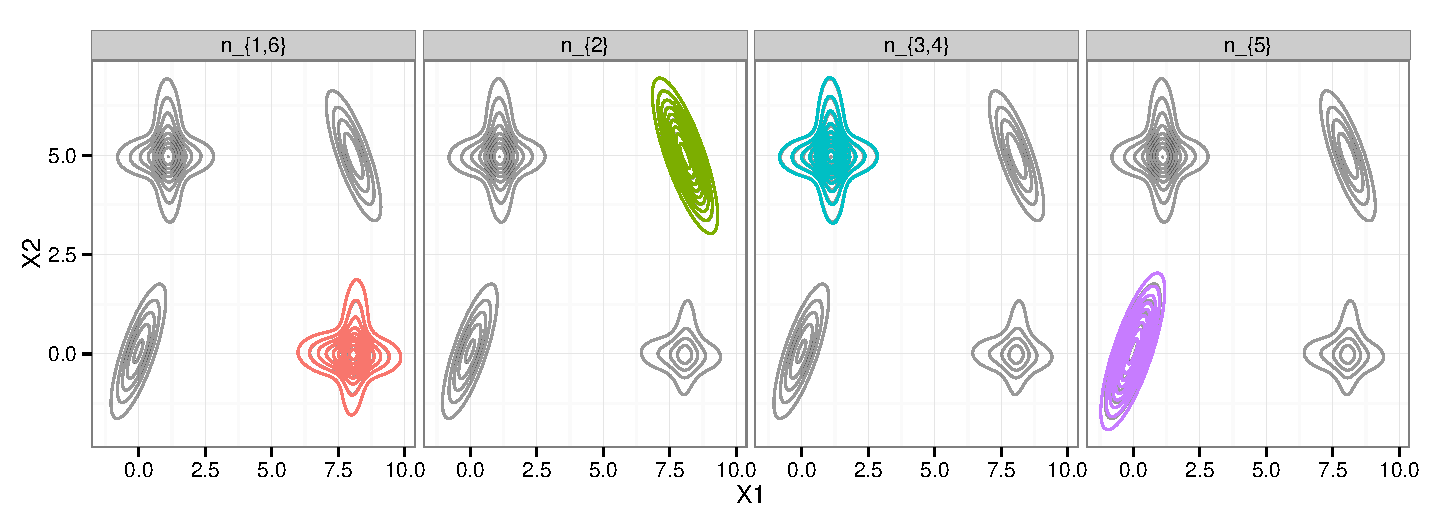
\includegraphics[width=\textwidth]{figures/baudry_ex4_1_all_distributions_4c.pdf}

\uncover<3->{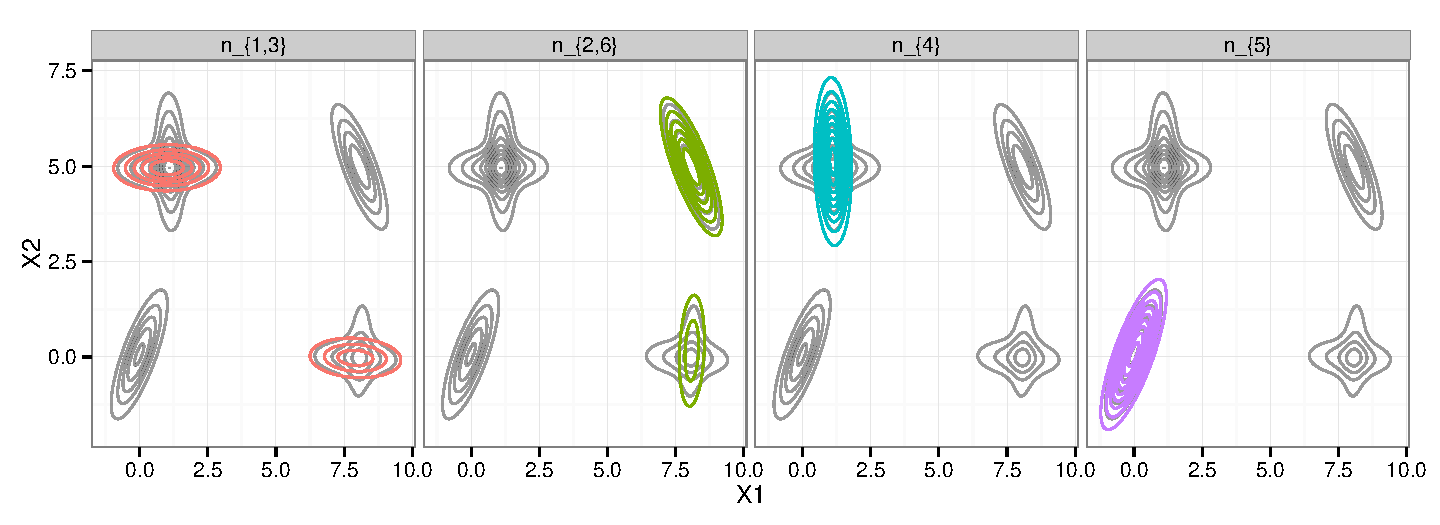
\includegraphics[width=\textwidth]{figures/baudry_ex4_1_all_distributions_4c_b.pdf}}
}

\column{0.6\textwidth}
\small
\begin{itemize}
\item Maybe one cluster is better explained as one mixture of components (``mixture of mixtures'')
\item<2-> From a likelihood point of view it is not possible to choose which ``mixture of mixtures'' is better.
\item<3-> Non-identificability: Both mixtures have the same likelihood.
\item<4> Different authors propose methods to merge components two by two.
\item<4> Here we focus on those methods based on posteriori probabilities which combines the components hierarchically.
\end{itemize}
\end{columns}
\end{frame}

\begin{frame}[t]
\frametitle{Mixture models: hierarchical component merging}
\begin{columns}[T]
\column{0.5\textwidth}
\small
Starting from a mixture model where each component is a cluster

\medskip

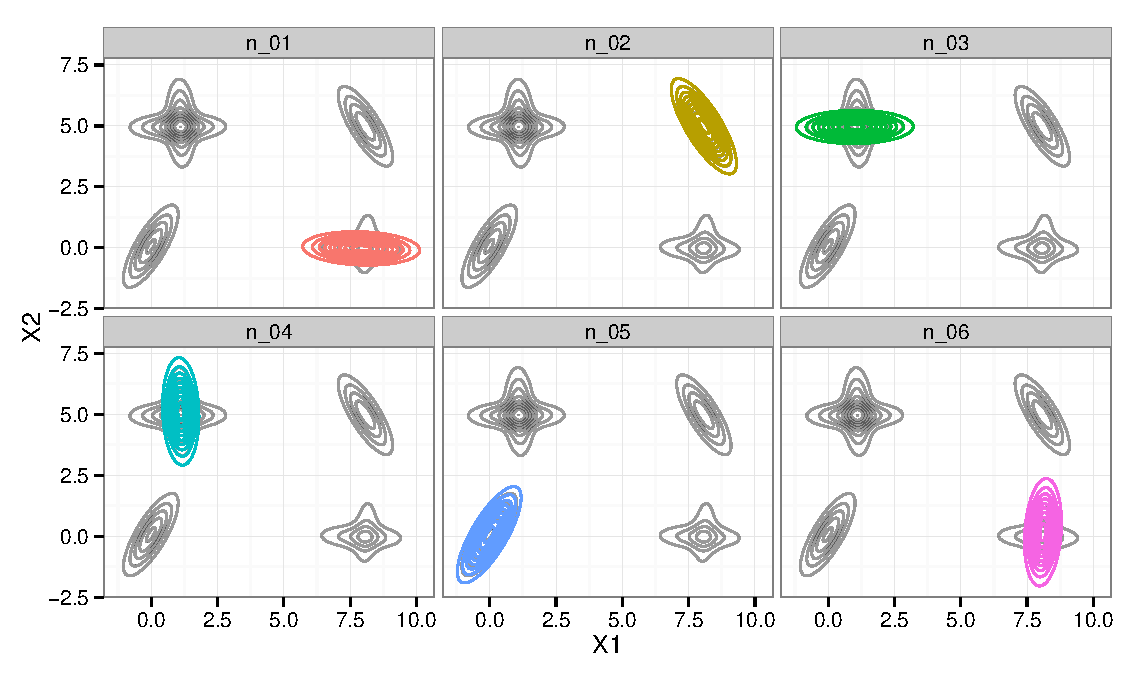
\includegraphics[width=0.9\textwidth]{figures/baudry_ex4_1_all_distributions.pdf}

combine sequentially the components to obtain a hierarchy over the set of components.

\pause
\column{0.5\textwidth}
\centering
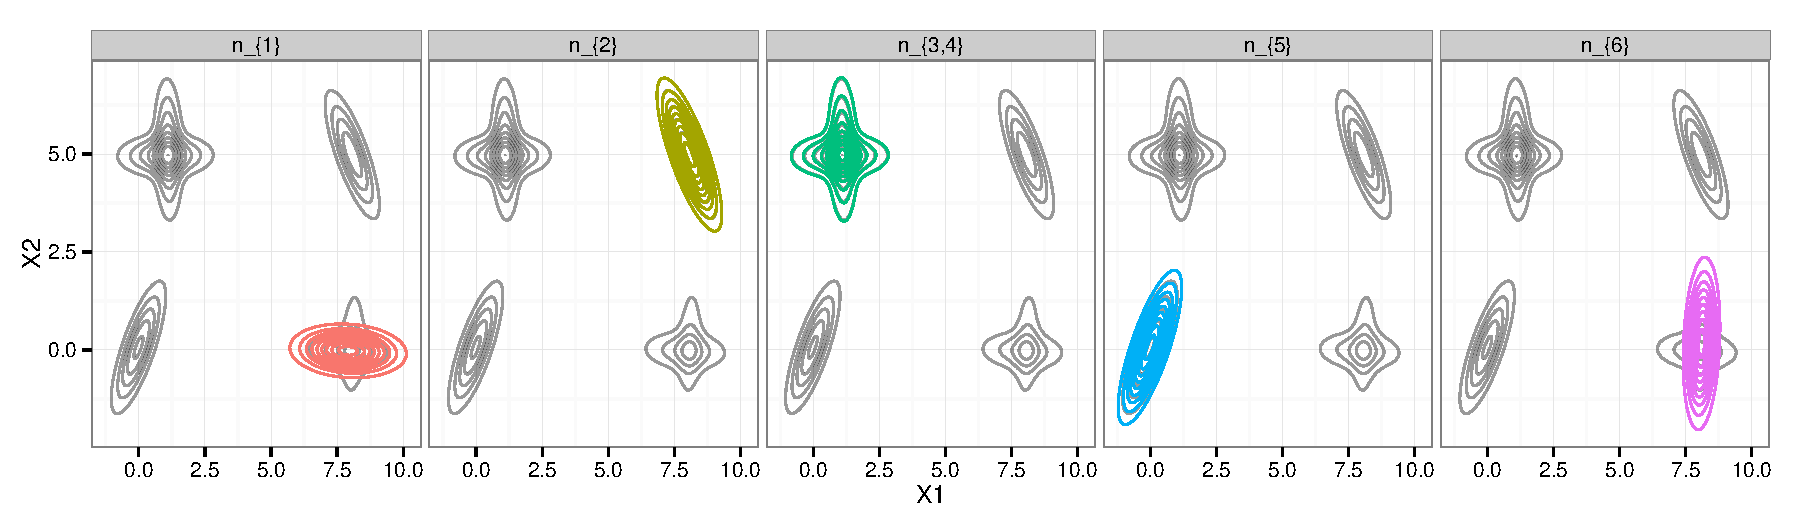
\includegraphics[height=0.2\textheight]{figures/baudry_ex4_1_all_distributions_5c.pdf}

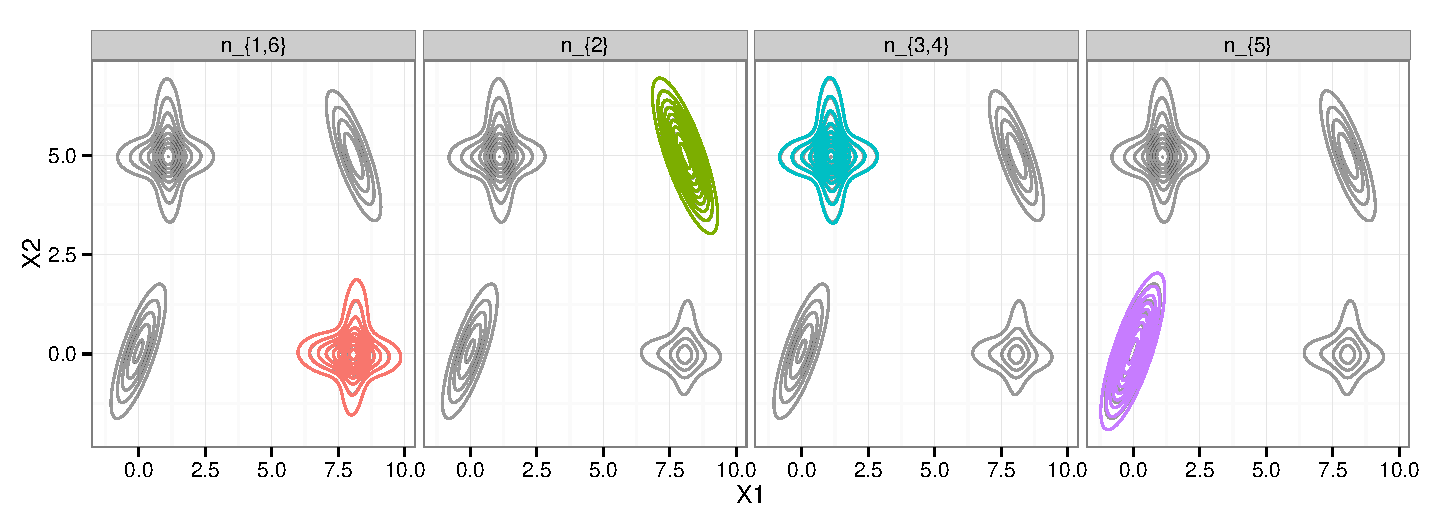
\includegraphics[height=0.2\textheight]{figures/baudry_ex4_1_all_distributions_4c.pdf}

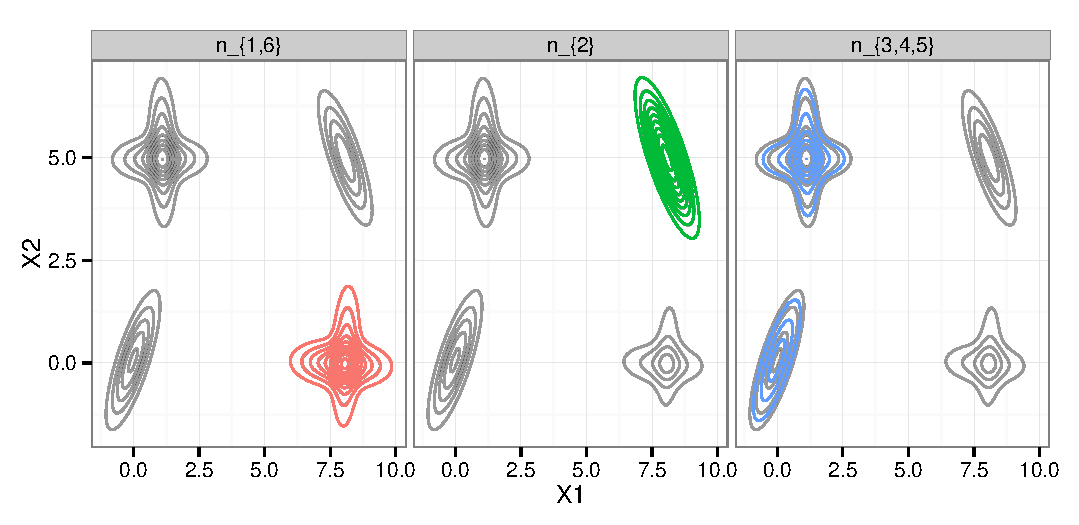
\includegraphics[height=0.2\textheight]{figures/baudry_ex4_1_all_distributions_3c.pdf} 

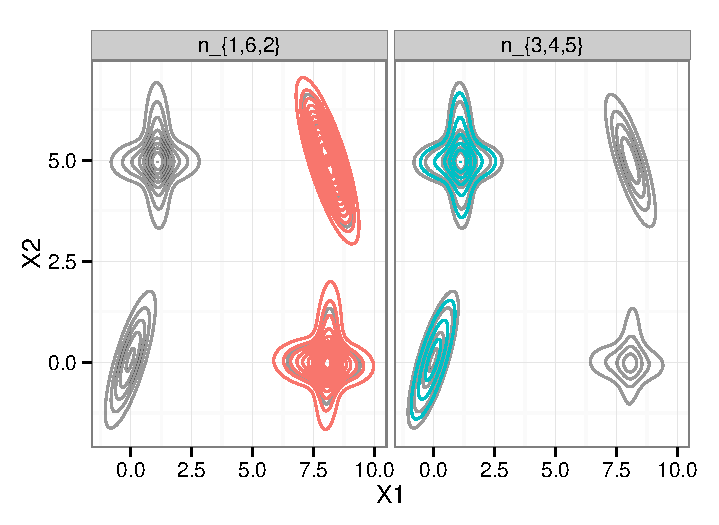
\includegraphics[height=0.2\textheight]{figures/baudry_ex4_1_all_distributions_2c.pdf}
\end{columns}
\end{frame}

\begin{frame}[t]
\frametitle{Our input, our goal: What do we want to do?}

\begin{block}{Input}
A sample of probabilities to belong to each component $C_i$, 
\begin{columns}
\column{0.4\textwidth}
\[ T = \left[ \begin{array}{ccccc}
\idea{(}\tau_{11}\idea{,} & \dots & \tau_{1j}\idea{,} & \dots & \tau_{1k}\idea{),} \\
\vdots      & &    \vdots                     & &    \vdots                     \\
\idea{(}\tau_{i1}\idea{,} & \dots & \tau_{ij}\idea{,} & \dots & \tau_{ik}\idea{),} \\
\vdots      & &      \vdots                   & &       \vdots                  \\
\idea{(}\tau_{n1}\idea{,} & \dots & \tau_{nj}\idea{,} & \dots & \tau_{nk}\idea{)}
\end{array} \right] 
\idea{ \in \mathcal{S}_{[C_1,\dots,C_k]}^k } \]
\column{0.3\textwidth}
\end{columns}
\end{block}

\pause
\begin{alertblock}{Goal}
\alert{Merge} components (sequentially) to obtain a hierarchy over the set of components % $\{C_1, \dots, C_k\}$. %In other words, obtain a binary tree with a set of leafs $\{C_1, \dots, C_k\}$
\end{alertblock}
\end{frame}

%%% Mixture models
\section{Combining components}
\frame{\sectionpage}

\begin{frame}
\frametitle{Whats does "merge" usually mean  in mixture modeling?}
\begin{itemize}
\item Merging component $C_a$ with component $C_b$ to a new component $C_c$ means that observation related to component $C_{ab}$ either is related to component $C_a$ or to component $C_b$.
\item Mixture models assume that an observation comes from a unique component (belongs to a unique component).
\item For an observation $\textbf{x}_i$ 
\begin{eqnarray*} 
\uncover<2>{ \tau_{i c}  \;=\;} P( \{ \textbf{x}_i \in C_{c} \})  &=& P( \{ \textbf{x}_i \in C_{a} \} \cup \{ \textbf{x}_i \in C_{b} \} ) \\
&=& P( \{ \textbf{x}_i \in C_{a} \}) + P( \{ \textbf{x}_i \in C_{b} \} )  \uncover<2>{ \;=\; \tau_{i a} + \tau_{i b} }
\end{eqnarray*} 
\end{itemize}
\end{frame}

\begin{frame}[t]
\frametitle{Entropy approach}
\begin{block}{Entropy approach (Baudry et~al., 2010)}
The components to be merged are those that maximize the entropy of a posteriori probabilities
\end{block}
\small
\only<1-2>{
\uncover<2>{Maximize}
\[
\overbrace{ 
\uncover<2>{-\left(} \sum_{i=1}^n \left\{ \tau_{i a} \log(\tau_{i a}) + \tau_{i b} \log(\tau_{i b})\right\} + \sum_{i=1}^n \sum_{\substack{\ell = 1\\\ell \neq a,b}}^k  \tau_{i \ell} \log(\tau_{i \ell}) \uncover<2>{\right)+}
}^{
\substack{\text{entropy }\\\text{before merging}}  
} 
\]
\[
\underbrace{ 
\uncover<2>{+\left( } \sum_{i=1}^n  (\tau_{i a}+\tau_{i b}) \log(\tau_{i a} + \tau_{i b}) + \sum_{i=1}^n  \sum_{\substack{\ell = 1\\\ell \neq a,b}}^k  \tau_{i \ell} \log(\tau_{i \ell}) \uncover<2>{\right)}
}_{
\substack{\text{entropy }\\\text{after merging}}   
} 
\]
}
\only<3>{
Maximize
\[
- \sum_{i=1}^n \left\{ \tau_{i a} \log(\tau_{i a}) + \tau_{i b} \log(\tau_{i b})\right\} + \sum_{i=1}^n  (\tau_{i a}+\tau_{i b}) \log(\tau_{i a} + \tau_{i b})
\]
}
%\only<4>{
%Minimize
%\[
% \sum_{i=1}^n \left\{ \tau_{i a} \log(\tau_{i a}) + \tau_{i b} \log(\tau_{i b})\right\} - \sum_{i=1}^n  (\tau_{i a}+\tau_{i b}) \log(\tau_{i a} + \tau_{i b})
%\]
%}
\end{frame}

\begin{frame}
\frametitle{Directly estimated misclassification probabilities (DEMP)}
\small
\begin{block}{DEMP approach (Hennig, 2010)}
The components to be merged are those that maximize the misclassification probability
\[
P\left( \{ \widetilde{\gamma}(x_i) = a \} | \{ \gamma(x_i) = b \} \right)
\]
\[
\begin{array}{rcl}
\{ \gamma(x_i) = b \} &:=& \text{\emph{``$x_i$ comes from component $b$''}} \text{ and} \\
\{\widetilde{\gamma}(x_i) = a\} &:=& \text{\emph{``$x_i$ is classified at component $a$''}}
\end{array}
\]
\end{block}

\[
P\left( \{ \widetilde{\gamma}(x_i) = a \} \cap \{ \gamma(x_i) = b\} \right) \;=\; 
\frac{1}{n}%
\sum_{h=1}^n P( \{ \gamma(x_h) = b \} | x_h) 
\mathbbm{1}\left( \{ \widetilde{\gamma}(x_n) = a \} \right)
\]

Maximizing%
\[
\frac{P\left( \{ \widetilde{\gamma}(x_i) = a \} \cap \{ \gamma(x_i) = b \} \right)}{ P\left( \{ \gamma(x_i) = b \} \right) } = 
\frac{%
  \frac{1}{n}%
  \sum_{h=1}^n \tau_{hb}
  \mathbbm{1}\left( \{ \forall \ell \; \tau_{ha} \geq \tau_{h\ell}  \} \right)
}{%
  \pi_b
}
\]
\end{frame}

\begin{frame}[t]
\frametitle{Log-ratio approach}
\small
\begin{block}{Log-ratio approach (ERCIM'13)}
The components to be merged are those that minimize
\[
\frac{1}{n_a} \sum_{x_i \in G_a}%
\only<1,3>{\left\| (\tau_{ia}, \tau_{ib}) \right\|_{\mathcal{A}}}%
\only<2>{\frac{1}{\sqrt{2}} \log (\frac{\tau_{ia}}{\tau_{ib}})}
\mathbbm{1}\left( \{ \forall \ell \; \tau_{ha} \geq \tau_{h\ell}  \}\right)
\]
\[\begin{array}{rcl}
G_a &:=& \text{ elements classified to component $a$ } \\
n_a &:=& \text{ number of elements classified to component $a$ }
\end{array}\]
\end{block}


\begin{itemize}
\item As DEMP approach, the log-ratio approach is not symmetric. 
\item Lower values of $\left\| (\tau_{ia}, \tau_{ib}) \right\|_{\mathcal{A}}$ means that the confusion between component $a$ and $b$ is high.
\end{itemize}

\end{frame}

\begin{frame}
\frametitle{Methods summary}
\small
\begin{tabular}{ >{\centering}m{0.7in} | >{\centering}m{0.8in} | >{\centering}m{1.3in} m{0in}}
\textbf{Method} & \textbf{optimization} & \textbf{criteria} & \\\hline\hline
Entropy     & max  & 
$\substack{- \sum_{i=1}^n \left\{ \tau_{i a} \log(\tau_{i a}) + \tau_{i b} \log(\tau_{i b})\right\} + \\
\sum_{i=1}^n  (\tau_{i a}+\tau_{i b}) \log(\tau_{i a} + \tau_{i b})}$  & \\ [2em]
\hline
DEMP        & max & $\frac{ \frac{1}{n} \sum_{h=1}^n \tau_{hb} \mathbbm{1}\left( \{ \forall \ell \; \tau_{ha} \geq \tau_{h\ell}  \} \right) }{ \pi_b }$ &\\ [2em]
\hline
Log-ratio   & min & $\frac{1}{n_a} \sum_{x_i \in G_a} \left\| (\tau_{ia}, \tau_{ib}) \right\|_{\mathcal{A}}$ & \\ [2em]
\end{tabular}

\end{frame}

\begin{frame}[fragile]
\frametitle{Comparing methods using Rand Index}
\centering
\begin{columns}[T]
\column{0.5\textwidth}
\uncover<2>{\includegraphics[width=\textwidth]{pdf/comparing-three-methods.pdf}}

\column{0.5\textwidth}
\scriptsize


\textbf{Simulation:}

\begin{itemize}
\item $f_i$: 100 gaussian mixture with $3$ components with $\omega \in \{ 0.01, 0.02, 0.04, 0.08, 0.16, 0.32\}$
\item Two gaussian mixture with 9 components are fitted to a sample coming from $f_i$ (spherical \& unrestricted) 
\item Using each method $(100 \times 6 \times 2)$, a component hierarchy is calculated
\item Level $3$ of hierarchy is compared to the initial cluster using Rand Index.
% ( $100 \times 6 \times 2$ simulations for each method )
\end{itemize}
\medskip
\medskip

\pause
\begin{verbatim}
             entropy   demp  atchison
  omega=0.01  0.8120 0.9294    0.9874
  omega=0.02  0.7295 0.8902    0.9732
  omega=0.04  0.6193 0.8614    0.9412
  omega=0.08  0.4893 0.7901    0.8813
  omega=0.16  0.3314 0.6464    0.7320
  omega=0.32  0.2103 0.4327    0.5083
\end{verbatim}

\end{columns}

\end{frame}


\begin{frame}[t]
\frametitle{Main ideas behind log-ratio approach}
\small
Minimize
\begin{center}
\[
\frac{1}{n_a} \sum_{x_i \in G_a} \left\| (\tau_{ia}, \tau_{ib}) \right\|_{\mathcal{A}}  =
\frac%
{ \sum_{i=1}^n \mathlarger{\mathbbm{1}}\left\{ \forall \ell\; \; \tau_{ia} \geq \tau_{i\ell}  \right\} \left\| (\tau_{ia}, \tau_{ib}) \right\|_{\mathcal{A}}  }%
{ \sum_{i=1}^n \mathlarger{\mathbbm{1}}\left\{ \forall \ell\; \; \tau_{ia} \geq \tau_{i\ell}  \right\}  }
%\frac{1}{n_a} \sum_{x_i \in G_a} \left\| (\tau_{ia}, \tau_{ib}) \right\|_{\mathcal{A}}
\]
\end{center}
\begin{itemize}
\item A measure of dissimilarity between components.
\item Individuals classified to the component are used to calculate the ``difference''

\begin{itemize}
\item Dissimilarity between components: \[\left\| (\tau_{ia}, \tau_{ib}) \right\|_{\mathcal{A}}\]
\item Relevance of an individual to a component: \[\mathlarger{\mathbbm{1}}\left\{ \forall \ell\; \; \tau_{ia} \geq \tau_{i\ell} \right\} \]
\end{itemize}

\end{itemize}

\end{frame}

\begin{frame}
\frametitle{General approach}
\small

Minimize
\[
\frac{ 
\sum_{i=1}^n \omega(\boldsymbol\tau_i, a) \;\; \varphi(\boldsymbol\tau_i, a, b) 
}{ 
\sum_{i=1}^n \omega(\boldsymbol\tau_i, a)
}
\]

\begin{itemize}
\item Dissimilarity between components: 
\[ \varphi(\boldsymbol\tau_i, a, b) \;\;\;\;\;\;\;\;\;\;\;\; \idea{\text{   example: $\left\| (\tau_{ia}, \tau_{ib}) \right\|_{\mathcal{A}}$}} \]
\item Relevance of an individual to a component: \[ \omega(\boldsymbol\tau_i, a) \;\;\;\;\;\;\;\;\;\;\;\; \idea{\text{   example: $\mathlarger{\mathbbm{1}}\left\{ \forall \ell\; \; \tau_{ia} \geq \tau_{i\ell}  \right\}$}} \]
\end{itemize}

\end{frame}

\begin{frame}[t]
\frametitle{General approach: Entropy}
\small
\begin{columns}
\column{0.6\textwidth}
\begin{block}{General}
Minimize
\[
\frac{ 
\sum_{i=1}^n \omega(\boldsymbol\tau_i, a) \;\; \varphi(\boldsymbol\tau_i, a, b) 
}{ 
\sum_{i=1}^n \omega(\boldsymbol\tau_i, a)
}
\]
\end{block}

\medskip
\medskip

\begin{itemize}
\item Dissimilarity between components: 
\item[] $\; \varphi(\boldsymbol\tau_i, a, b) \uncover<3>{ =  \tau_{i a} \log(\tau_{i a}) + \tau_{i b} \log(\tau_{i b}) - (\tau_{i a}+\tau_{i b}) \log(\tau_{i a} + \tau_{i b})}$
\item Relevance of an individual to a component: 
\item[] $\; \omega(\boldsymbol\tau_i, a) \uncover<3>{ = 1}$
\end{itemize}


\column{0.4\textwidth}%
Maximize \[ \large\substack{- \sum_{i=1}^n \left\{ \tau_{i a} \log(\tau_{i a}) + \tau_{i b} \log(\tau_{i b})\right\} + \\\\
+ \sum_{i=1}^n  (\tau_{i a}+\tau_{i b}) \log(\tau_{i a} + \tau_{i b})} \]
\uncover<2->{%
\[ \Updownarrow \]
Minimize \[\large\substack{\sum_{i=1}^n \left\{ \tau_{i a} \log(\tau_{i a}) + \tau_{i b} \log(\tau_{i b})\right\} - \\\\
- \sum_{i=1}^n  (\tau_{i a}+\tau_{i b}) \log(\tau_{i a} + \tau_{i b})} \]}
\end{columns}

\end{frame} 


\begin{frame}[t]
\frametitle{General approach: DEMP}
\small
\begin{columns}
\column{0.6\textwidth}
\begin{block}{General}
Minimize
\[
\frac{ 
\sum_{i=1}^n \omega(\boldsymbol\tau_i, a) \;\; \varphi(\boldsymbol\tau_i, a, b) 
}{ 
\sum_{i=1}^n \omega(\boldsymbol\tau_i, a)
}
\]
\end{block}

\medskip
\medskip

\begin{itemize}
\item Dissimilarity between components: 
\item[] $\; \varphi(\boldsymbol\tau_i, a, b) \uncover<4>{ = \mathlarger{\mathbbm{1}}\left\{ \exists \ell \; \tau_{hb} < \tau_{h\ell}  \right\}}$
\item Relevance of an individual to a component: 
\item[] $\; \omega(\boldsymbol\tau_i, a) \uncover<4>{ = \tau_{ha}}$
\end{itemize}


\column{0.4\textwidth}%
Maximize \[ \frac{ \frac{1}{n} \sum_{h=1}^n \tau_{ha} \mathlarger{\mathbbm{1}}\left\{ \forall \ell\; \; \tau_{hb} \geq \tau_{h\ell}  \right\} }{ \pi_a } \]
\uncover<2->{%
\[ \Updownarrow \]
Maximize \[ \frac{ \frac{1}{n} \sum_{h=1}^n \tau_{ha} \mathlarger{\mathbbm{1}}\left\{  \forall \ell\; \; \tau_{hb} \geq \tau_{h\ell}  \right\} }{ \frac{1}{n} \sum_{h=1}^n \tau_{ha} } \]}
\uncover<3->{%
\[ \Updownarrow \]
Minimize \[ \frac{  \sum_{h=1}^n \tau_{ha} \mathlarger{\mathbbm{1}}\left\{  \exists \ell\; \; \tau_{hb} < \tau_{h\ell}  \right\}  }{  \sum_{h=1}^n \tau_{ha} } \]}
\end{columns}

\end{frame} 


\begin{frame}
\frametitle{Summarizing}
\scriptsize

\begin{tabular}{c  c | >{\centering}m{0.7in} | >{\centering}m{0.7in} | >{\centering}m{0.7in} | m{0in}} 
 & \multicolumn{1}{c}{} & \multicolumn{3}{c}{$\omega(\boldsymbol\tau_i, a)$} &\\
 & \multicolumn{1}{c}{} & \multicolumn{1}{c}{} & \multicolumn{1}{c}{} & \multicolumn{1}{c}{} & \multicolumn{1}{c}{}\\
 & \multicolumn{1}{c}{} & \multicolumn{1}{c}{1} & \multicolumn{1}{c}{$\tau_{ia}$} & \multicolumn{1}{c}{$\mathlarger{\mathbbm{1}}\left\{  \forall \ell\; \; \tau_{ia} \geq \tau_{i\ell}  \right\}$} &\\ \cline{3-5} 
 & $\large\substack{\tau_{i a} \log(\tau_{i a}) + \tau_{i b} \log(\tau_{i b}) - \\ - (\tau_{i a}+\tau_{i b}) \log(\tau_{i a} + \tau_{i b})}$ & Entropy & \uncover<2->{\red{prop-entropy}} &  \uncover<2->{\red{dicho-entropy}} &\\[5em] \cline{3-5}
\rotatebox[origin=c]{90}{$\varphi(\boldsymbol\tau_i, a, b)$} & $\mathlarger{\mathbbm{1}}\left\{  \exists \ell \; \tau_{hb} < \tau_{h\ell}  \right\}$ & \uncover<2->{\red{const-DEMP}} & DEMP  & \uncover<2->{\red{dicho-DEMP}} & \\[5em] \cline{3-5}
& $\log{\tau_{i a} / \tau_{i b}}$ & \uncover<2->{\red{const-Log-ratio}} & \uncover<2->{\red{prop-Log-ratio \\(Kullback-Leibler)}} &  Log-ratio &\\[5em] \cline{3-5}
\uncover<3>{& $-\tau_{i b}$ & \red{??} & \red{prop-DEMP} &  \red{??} &\\[5em] \cline{3-5}}
\end{tabular}

% \begin{tabular}{ >{\centering}m{0.7in} | >{\centering}m{0.8in} | >{\centering}m{1.3in} m{0in}}
% \textbf{Method} & \textbf{optimization} & \textbf{criteria} & \\\hline\hline
% Entropy     & max  & 
% $\substack{- \sum_{i=1}^n \left\{ \tau_{i a} \log(\tau_{i a}) + \tau_{i b} \log(\tau_{i b})\right\} + \\
% \sum_{i=1}^n  (\tau_{i a}+\tau_{i b}) \log(\tau_{i a} + \tau_{i b})}$  & \\ [2em]
% \hline
% DEMP        & max & $\frac{ \frac{1}{n} \sum_{h=1}^n \tau_{hb} \mathlarger{\mathbbm{1}}\left( \{ \forall \ell \; \tau_{ha} \geq \tau_{h\ell}  \} \right) }{ \pi_b }$ &\\ [2em]
% \hline
% Log-ratio   & min & $\frac{1}{n_a} \sum_{x_i \in G_a} \left\| (\tau_{ia}, \tau_{ib}) \right\|_{\mathcal{A}}$ & \\ [2em]
% \end{tabular}
\end{frame}

\begin{frame}
\frametitle{Results}
\tiny
\begin{center}
\includegraphics[width=0.85\textwidth]{pdf/experiment04b.pdf}

\begin{tabular}{rrrrrrrr}
\hline\hline
\multicolumn{1}{c}{overlap}&\multicolumn{1}{c}{entropy}&\multicolumn{1}{c}{prop.entropy}&\multicolumn{1}{c}{dich-entropy}&\multicolumn{1}{c}{dich-aitchison}&\multicolumn{1}{c}{prop-aitchison}&\multicolumn{1}{c}{demp}&\multicolumn{1}{c}{prop-demp}\tabularnewline
\hline
$0.01$&$0.8120$&$0.9780$&$0.9790$&$0.9874$&$0.9877$&$0.9294$&$0.9694$\tabularnewline
$0.02$&$0.7295$&$0.9525$&$0.9517$&$0.9732$&$0.9733$&$0.8902$&$0.9407$\tabularnewline
$0.04$&$0.6193$&$0.9234$&$0.9211$&$0.9412$&$0.9420$&$0.8614$&$0.9111$\tabularnewline
$0.08$&$0.4893$&$0.8633$&$0.8626$&$0.8813$&$0.8811$&$0.7901$&$0.8410$\tabularnewline
$0.16$&$0.3314$&$0.7207$&$0.7235$&$0.7320$&$0.7320$&$0.6464$&$0.6886$\tabularnewline
$0.32$&$0.2103$&$0.4966$&$0.5024$&$0.5083$&$0.5063$&$0.4327$&$0.4668$\tabularnewline
\hline
\end{tabular}\end{center}
\end{frame}

%%% Further work
\section{Merging classes}
\frame{\sectionpage}

\begin{frame}
\frametitle{Whats does "merge" usually mean  in general?}
%\frametitle{Merging operation}


\begin{itemize}
\item What if we apply geometric mean instead of amalgamation
\end{itemize}
\end{frame}

\begin{frame}
\frametitle{Ideas}
\begin{itemize}
\item Usually, we assume our sample $X$ to be near to the center of a class. Is this assumption really important to merge clusters?
\end{itemize}
\end{frame}

%%%%%%%%%%%%%
%%% Last part
\section{Conclusions}
\begin{frame}
\frametitle{Conclusions}
\begin{itemize}
\item Our approach works with compositions. This allows us to define generic methods for different problems in a common framework.
\item From a simulation study, 
\begin{itemize}
\item entropy does not work properly when the level of overlapping increase and
\item From a simulation study, those methods based on Log-ratio approach seems to work lightly better than methods based on DEMP approach.
\end{itemize}
\item Modifying the merging methodology we can build a hierarchy over the components of a compositional sample. Can be this hierarchy useful to define a binary partition with ``good'' properties? 
\end{itemize}

\end{frame}

\begin{frame}[plain]

  \begin{columns}
    \begin{column}{0.65\textwidth}
      \begin{center}

        \font\endfont = cmss10 at 15.40mm
        
        \endfont 
        \baselineskip 15.0mm

        Gr\`{a}cies!!!

      \end{center}    

    \end{column}
    \begin{column}{0.35\textwidth}
      \begin{center}
        \pgfimage[width=\textwidth]{tern.png}          
      \end{center}
    \end{column}
  \end{columns}

\end{frame}
%\begin{frame}[t]
\frametitle{Fuzzy clustering VS Mixture modeling}

% \begin{columns}
% \column{0.5\textwidth}
% \begin{itemize}
% \item 
% \end{itemize}
% \column{0.5\textwidth}
% \begin{itemize}
% \item 
% \end{itemize}
% \end{columns}

\begin{columns}
\column{0.5\textwidth}
Fuzzy-clustering\medskip
\begin{itemize}
\item Initialize $(\omega_{i1}^0, \dots, \omega_{ik}^0)$.
\end{itemize}
\column{0.5\textwidth}

Gaussian mixture modeling\medskip
\begin{itemize}
\item Initialize $(\tau_{i1}^0, \dots, \tau_{ik}^0)$.
\end{itemize}
\end{columns}

\begin{columns}
\column{0.5\textwidth}
\begin{itemize}
\item $c^{\ell+1}_j = \frac{\sum_{i=1}^n \omega_{i j}^{\red{m}} \obs{x_i}}{\sum_{i=1}^n \omega_{i j}^{\red{m}}}$
\end{itemize}
\column{0.5\textwidth}
\begin{itemize}
\item $\mu^{\ell+1}_j = \frac{\sum_{i=1}^n \tau_{i j} \obs{x_i}}{\sum_{i=1}^n \tau_{i j}}$
\end{itemize}
\end{columns}

\begin{columns}
\column{0.5\textwidth}
\begin{itemize}
\item $\omega^{\ell+1}_{ij} = \frac{1}{\sum_{\ell = 1}^k \left( \frac{d(x_i; C_j)}{d(x_i; C_\ell) } \right)^{2/({\red{m}}-1)}}$
\end{itemize}
\column{0.5\textwidth}
\begin{itemize}
\item $\tau^{\ell+1}_{ij} = \frac{f(x_i; \mu_j, \Sigma_\ell)}{\sum_{\ell = 1}^k f(x_i; \mu_\ell, \Sigma_\ell) }$
\end{itemize}
\end{columns}


\end{frame}
\end{document}